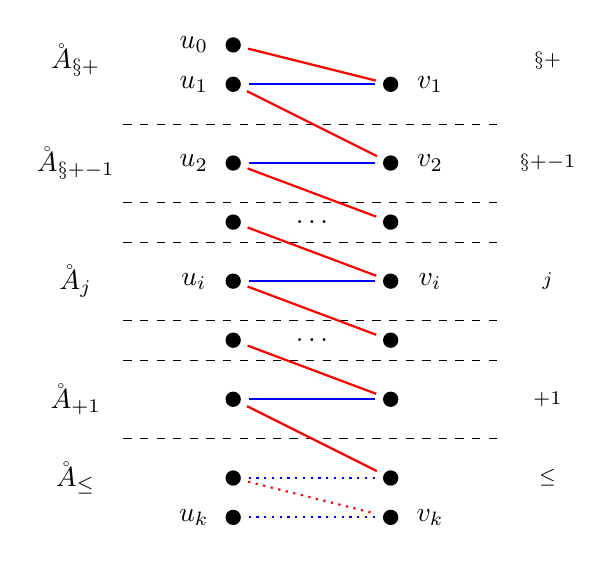
\begin{tikzpicture}[thick,
  lnode/.style={draw=white,fill=blue},
  fsnode/.style={draw,circle,fill=black,scale=0.5},
  every fit/.style={ellipse,draw,inner sep=-2pt,text width=0.5cm},
  -,shorten >= 3pt,shorten <= 3pt
]

% % the vertices of A U B
% \node at (0,1) {$\AA'$};
% \node at (2,1) {$\BB'$};

  \node[fsnode] (u0) at (0,0.5) {};
  \node at (-0.5,0.5) {$u_0$};
  \node[fsnode] (v1) at (2,0) {};
  \node at (2.5,0) {$v_1$};
  \node[fsnode] (u1) at (0,0) {};
  \node at (-0.5,0) {$u_1$};
  \node at (-2,0.3) {$\AA_{\S+\T}$};
  \node at (4,0.3) {$\BB_{\S+\T}$};
   \draw[ultra thin, dashed](-1.5,-0.5) -- (3.5,-0.5);
   
  \node[fsnode] (v2) at (2,-1) {};
  \node at (2.5,-1) {$v_2$};
  \node[fsnode] (u2) at (0,-1) {};
  \node at (-0.5,-1) {$u_2$};
   \node at (-2,-1) {$\AA_{\S+\T-1}$};
   \node at (4,-1) {$\BB_{\S+\T-1}$};
   \draw[ultra thin,dashed](-1.5,-1.5) -- (3.5,-1.5);
   
   \node[fsnode] (ui1) at (0,-1.75) {};
   \node[fsnode] (vi1) at (2,-1.75) {};
   \node at (1,-1.75) {$\ldots$};
   \draw[ultra thin,dashed](-1.5,-2) -- (3.5,-2);
   
  \node[fsnode] (vi) at (2,-2.5) {};
  \node at (2.5,-2.5) {$v_i$};
  \node[fsnode] (ui) at (0,-2.5) {};
  \node at (-0.5,-2.5) {$u_i$};
   \node at (-2,-2.5) {$\AA_{j}$};
  \node at (4,-2.5) {$\BB_{j}$};
   \draw[ultra thin, dashed](-1.5,-3) -- (3.5,-3);
   
   \node[fsnode] (ui11) at (0,-3.25) {};
   \node[fsnode] (vi11) at (2,-3.25) {};
   \node at (1,-3.25) {$\ldots$};
   \draw[ultra thin, dashed](-1.5,-3.5) -- (3.5,-3.5);

\node[fsnode] (vk1) at (2,-4) {};
 % \node at (2.7,-4) {$v_{k-1}$};
  \node[fsnode] (uk1) at (0,-4) {};
  %\node at (-0.6,-4) {$u_{k-1}$};
   \node at (-2,-4) {$\AA_{\T+1}$};
  \node at (4,-4) {$\BB_{\T+1}$};
   \draw[ultra thin, dashed](-1.5,-4.5) -- (3.5,-4.5);
   
   \node[fsnode] (vk) at (2,-5) {};
  %\node at (2.5,-5) {$v_{k}$};
  \node[fsnode] (uk) at (0,-5) {};
  %\node at (-0.5,-5) {$u_{k}$};
   \node at (-2,-5) {$\AA_{\le \T}$};
  \node at (4,-5) {$\BB_{\le \T}$};
  % \draw[ultra thin, dashed](-1.5,-5.5) -- (3.5,-5.5);
  
   % \node[fsnode] (vk11) at (2,-6) {};
  % \node at (2.7,-6) {$v_{k+1}$};
  %  \node at (-2,-6) {$\AA_{\T}$};
  % \node at (4,-6) {$\BB_{\T}$};
  \node[fsnode] (vk11) at (2,-5.5) {};
  \node at (2.5,-5.5) {$v_{k}$};
  \node[fsnode] (uk11) at (0,-5.5) {};
  \node at (-0.5,-5.5) {$u_{k}$};

% % the M edges
 \draw[thick, red ](u0) -- (v1);
 \draw[thick, blue](u1) -- (v1);
 \draw[thick, red ](u1) -- (v2);
 \draw[thick, blue](u2) -- (v2);
 \draw[thick, blue](ui) -- (vi);
 \draw[thick, red ](u2) -- (vi1);
 \draw[thick, red ](ui1) -- (vi);
 \draw[thick, red ](ui) -- (vi11);
 \draw[thick, red ](ui11) -- (vk1);
 \draw[thick, blue](uk1) -- (vk1);
 \draw[thick, red ](uk1) -- (vk);
 \draw[thick, dotted,blue](uk) -- (vk);
 \draw[thick, dotted, red ](uk) -- (vk11);
 \draw[thick, dotted,blue](uk11) -- (vk11);

%  \draw[dashed](g0) -- (h1);
%  \draw[dashed](g1) -- (h2);
%  \draw[dashed](gi) -- (hi1);
% \draw[dashed](g1') -- (h0);
% \draw[dashed](g2') -- (h1');
% \draw[dashed](gi1') -- (hi');
\end{tikzpicture}